\chapter{Reality}

\section{The Question of Reality}

In the book \textit{The Nature of Space and Time}, Roger Penrose and Stephen Hawking present two contrasting views on the nature of reality.

Penrose argues that there exists an objective reality independent of observation. In this view, the task of physics is to uncover what is truly there, whether or not we happen to be looking.

Hawking, by contrast, takes a more pragmatic stance. According to what is often called \emph{model-dependent realism}, we do not have access to reality ``as it is.''
Instead, we construct mathematical models and judge them by how well they predict observations. If a model works, we keep it. If it fails, we replace it. Reality, in this sense, is what survives experimental testing.

If so, then what is it that we sense as reality? And what is that we use for modelign the reality - mathematics?


\section{Classifying Attributes}

One way to approach this question is to separate the ingredients of our physical theories into three broad categories.

First, there are \emph{directly observable quantities}: detector clicks, positions on a screen, numbers printed by measuring devices.

Second, there are \emph{derived quantities}, such as energy. These are not directly observed, but inferred through consistent relationships like conservation laws.

Third, there are \emph{purely abstract constructs}: mathematical objects that exist only within the formalism of the theory.

At first glance, this seems like a reasonable hierarchy. What we can touch and measure feels real. What we calculate feels slightly less so. What exists only in equations feels, perhaps, suspiciously abstract.

But this intuition quickly begins to break down.


\section{A Rock, Some Energy, and an Unfortunate Toe}

Consider a one-kilogram rock. It feels undeniably real. If you drop it on your foot, the experience will strongly reinforce this belief.

Now lift that rock by one meter. In Earth's gravitational field, you have increased its potential energy by approximately 9.81 joules.

This energy cannot be seen, touched, or directly measured. There is no ``energy particle'' hiding inside the rock waiting to be inspected.
And yet, when the rock falls back down and lands on your toe, the result is both measurable and memorable.

One might say that 9.81 joules is an abstract bookkeeping device.

One's toe, however, may disagree.

The point is not that energy is unreal. On the contrary, it is one of the most precisely defined and reliably conserved quantities in physics.
The point is that even very ``real'' phenomena rely on quantities that are not themselves directly observable.

Already, the boundary between the real and the abstract begins to blur.


\section{Relativity and What Is ``Really'' There}

Relativity deepens this ambiguity.

The search for the "luminiferous ether" was one of the biggest scientific quests of the 19th century. Physicists back then couldn't imagine how light waves could travel through a total vacuum.
Just as sound needs air and ocean waves need water, they assumed light needed an invisible, weightless substance filling all of space: the ether.
In 1905 Einstein published his paper on Special Relativity. He realized that if one just assumed the speed of light is constant for everyone, one didn't need the ether at all.
He essentially "deleted" it from the map of the universe.

In special relativity, mass and energy are related by the equation \( E = mc^2 \). What we once thought of as distinct concepts turn out to be interchangeable.

In general relativity, the situation becomes even more unusual. Gravity is no longer a force acting at a distance, but a manifestation of the curvature of spacetime itself.
Massive objects distort geometry, and objects move along paths determined by that geometry.

So what is that geometry? 

It is nothing!

Spacetime curvature is not something that physically exists. It is part of the mathematical framework we use to describe motion. It is abstract.



\section{Quantum Mechanics and Abstract Machinery}

Quantum mechanics pushes abstraction even further.

The theory describes physical systems using a mathematical object called the wavefunction. This wavefunction is abstract by nature. It is not directly observable.
However, its squared magnitude determines probabilities of measurement outcomes.


\begin{figure}[h!]
\centering
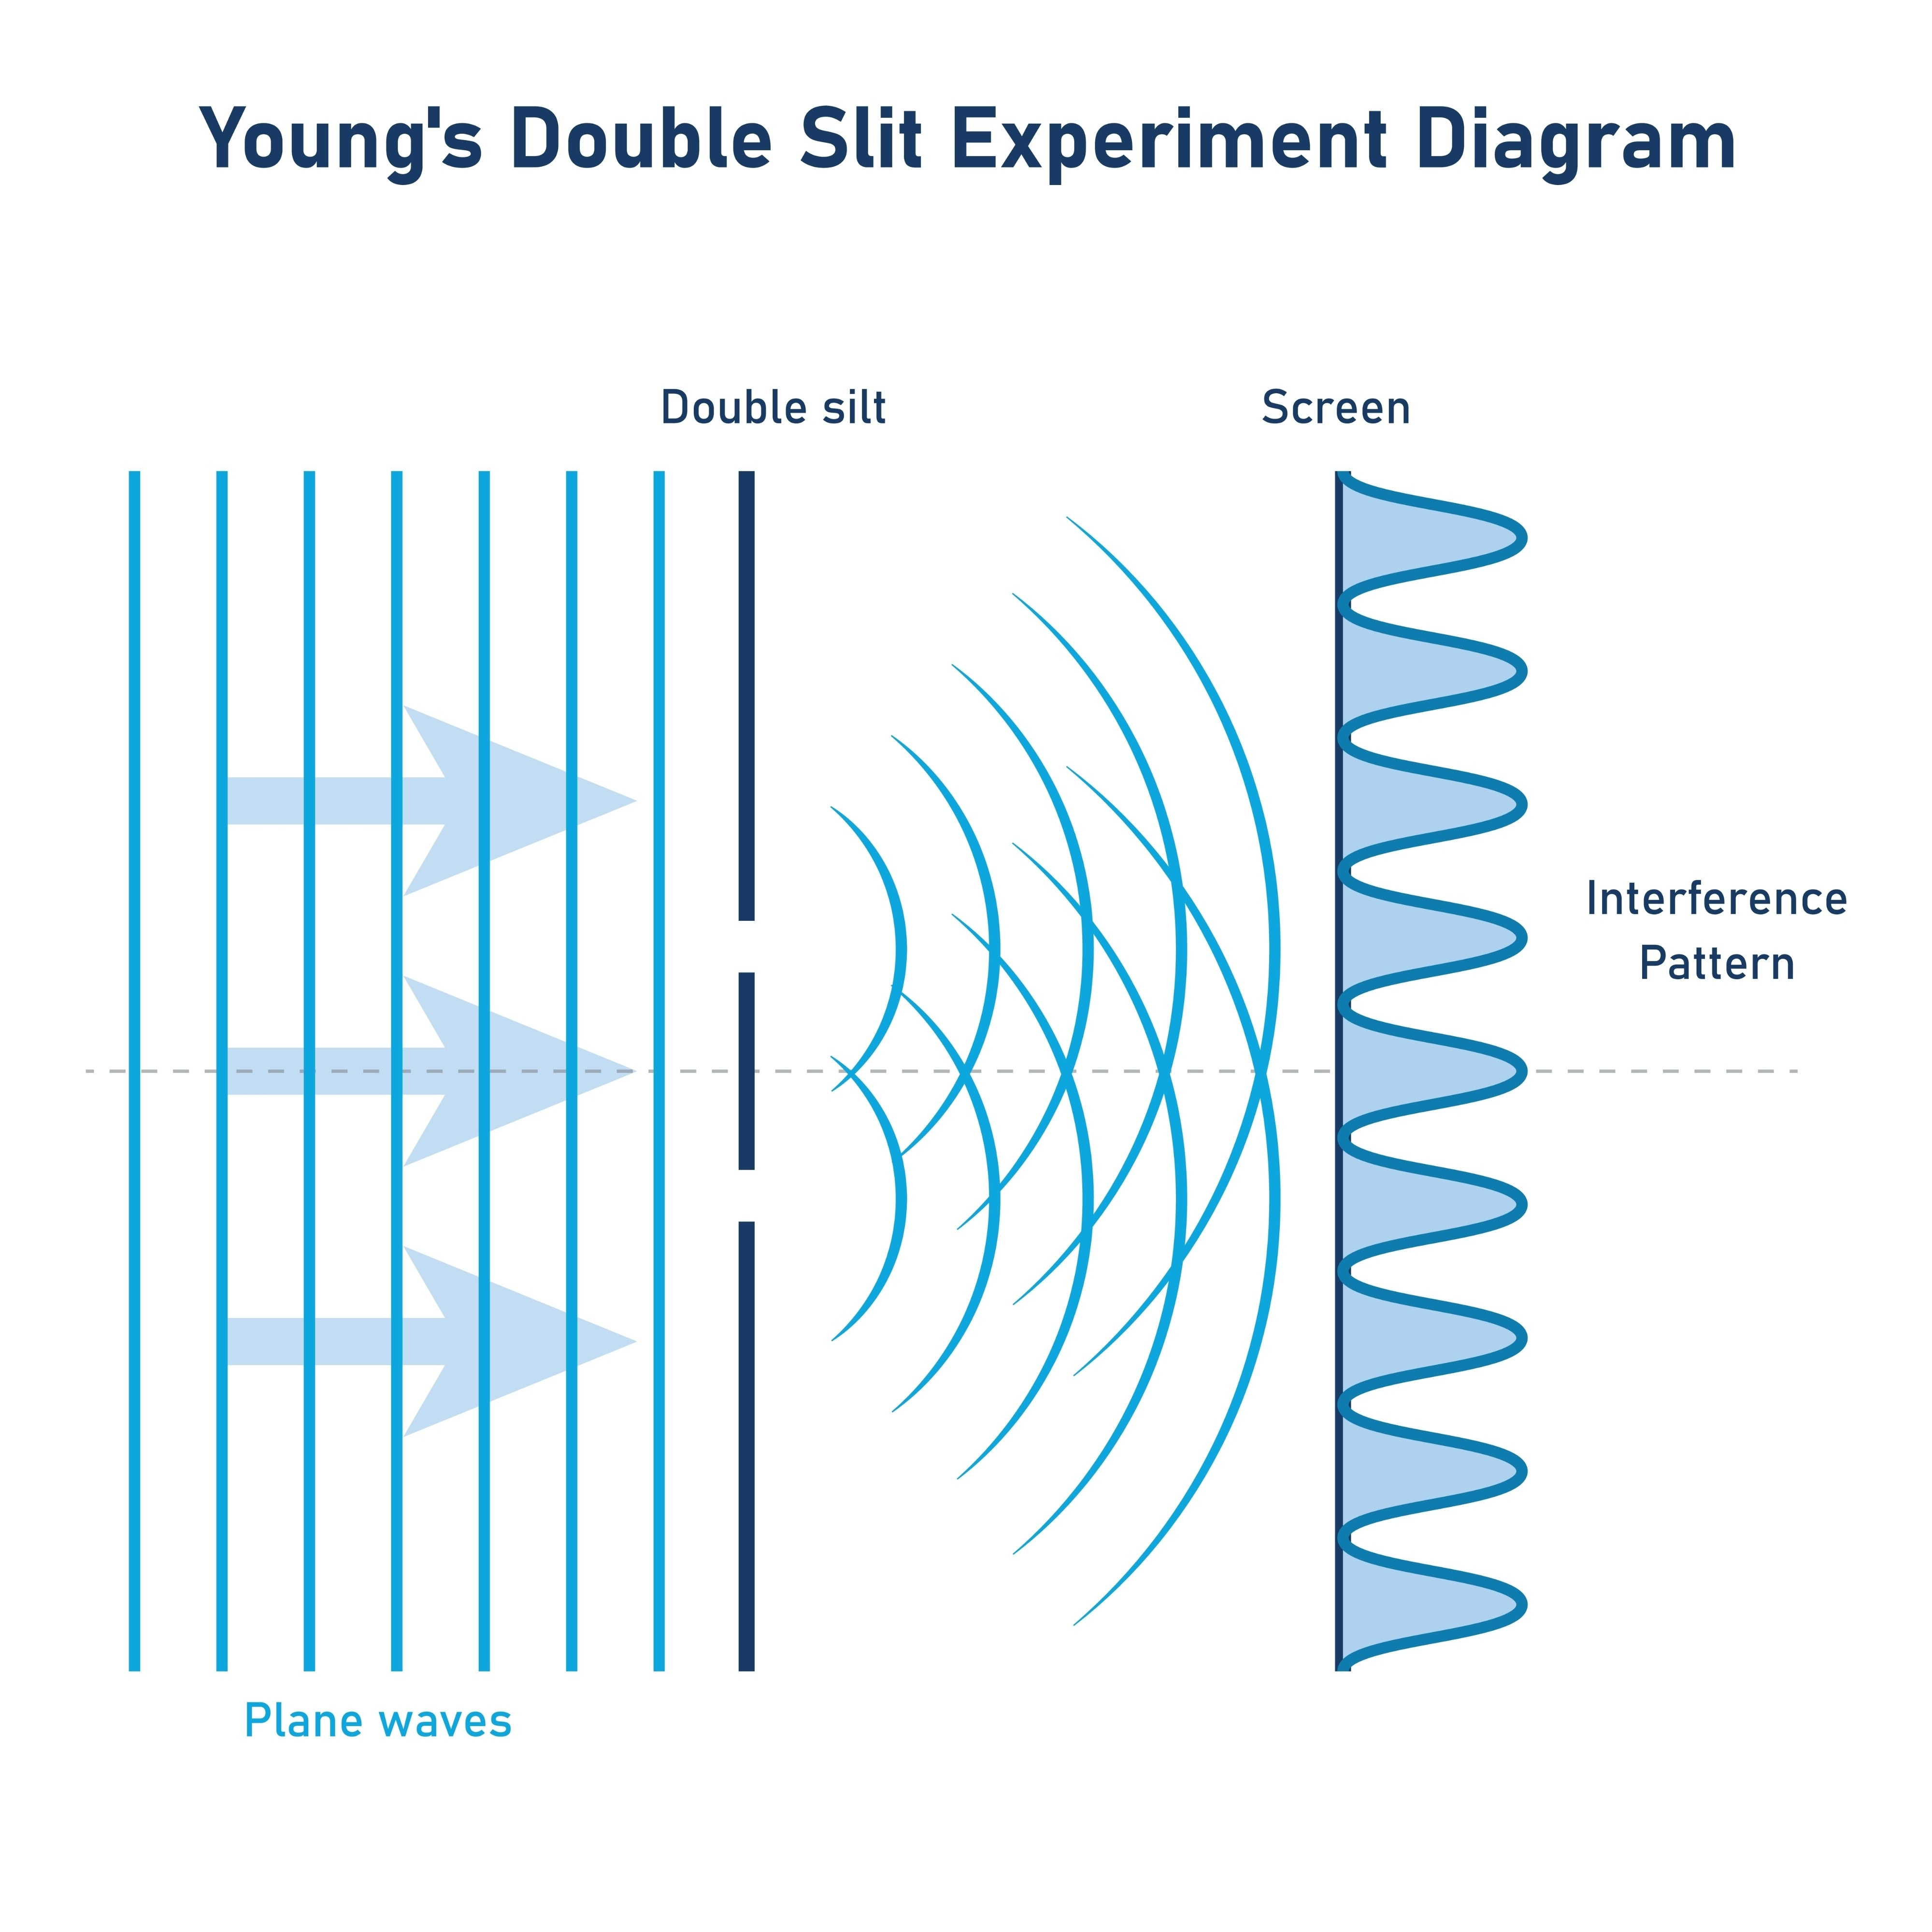
\includegraphics[width=0.8\textwidth]{figures/twoslitexperiment.jpg}
\caption{Observable result of the unobservable wavefunction}
\end{figure}


In modern formulations, what is called ``particles'' are excitations of underlying fields.
Some of these, such as photons, can be directly detected.
Others reveal themselves only indirectly through their effects.

The central machinery of the theory operates entirely in an abstract mathematical space. Yet its predictions match experiments with extraordinary precision.
The most accurate physical theory ever constructed relies fundamentally on entities that cannot themselves be observed.

How can purely abstract entity have total control over matter and energy? 


\section{Elusive Reality}

The unification of physics makes the problem even harder. Attempts to unify general relativity and quantum mechanics have led to increasingly
abstract mathematical frameworks. Far from eliminating abstraction, progress in physics seems to require more of it.

If abstract mathematical structures were only convenient fictions, we might expect that, with sufficient effort, they could be eliminated in favor of purely concrete descriptions.
But this does not appear to be the case.

If even a small part of our most successful description of the universe is irreducibly abstract, then a natural question arises, why should the rest of reality be any different?


